\chapter{向量与向量运算}
在常用的数量问题中,我们用数去表达各种量,如重
量、长度、面积、体积、密度等等;用加、减、乘、除运算
的组合去表达各种量之间的关系(通称代数通性)。在代数
中,我们已掌握了数系的基本性质(即交换律、结合律和分
配律)。并熟知了代数学的基本精神在于有效地运用数系
通性,对于各种类型的代数问题谋求通解(即以通性求通
解)。现在我们要着手把几何学的讨论也推进到定量的层
面,设法把空间结构有系统地代数化,数量化,这也就是本
章所要详加讨论的课题——\textbf{向量与向量运算}。为了便于同学
们逐步地理解向量这个基本概念,本章的前三节先对平面向
量详加分析,然后再在第四节讨论空间向量。

\section{平面位移向量及其加法运算}

\subsection{位移向量}

如图3.1所示,我们在$\overline{AB}$的端点$B$处画
上一个箭头表示 线段$\overline{AB}$具有射线$AB$的方向,这种用箭头指明方向的线段叫做\textbf{有向线段},记作$\Vec{AB}$,读作有向线段$AB$,并称A为$\Vec{AB}$的\textbf{始点},$B$为$\Vec{AB}$的\textbf{终点}。$\overline{AB}$的长叫做$\Vec{AB}$的长,并记作$|\Vec{AB}|$。

$\Vec{AB}$和$\Vec{CD}$同向且等长,那么我们称$\Vec{AB}$和$\Vec{CD}$\textbf{相等},记作$\Vec{AB}=\Vec{CD}$(图3.2)。

\begin{figure}[htp]\centering
    \begin{minipage}[t]{0.48\textwidth}
    \centering
\begin{tikzpicture}[>=latex, scale=.8]
    \draw[->](0,0)node[below]{$A$}--(2,3)node[above]{$B$};
    \end{tikzpicture}
    \caption{}
    \end{minipage}
    \begin{minipage}[t]{0.48\textwidth}
    \centering
    \begin{tikzpicture}[>=latex, scale=.8]
        \draw[->](0,0)node[below]{$A$}--(2,3)node[above]{$B$};
        \draw [dashed](0,0)--(3,.5);\draw [dashed](2,3)--(5,3.5);
        \draw[->](3,.5)node[below]{$C$}--(5,3.5)node[above]{$D$};
    \end{tikzpicture}
    \caption{}
    \end{minipage}
    \end{figure}

已知方向$ON$(图3.3), 如果平面上的每一点都沿射线
$ON$的方向移动相同的距离,那
么我们称这种平面上全体点的移
动叫做平面上全体点的一个\textbf{平移}。

\begin{figure}[htp]\centering
    \begin{minipage}[t]{0.48\textwidth}
    \centering
\begin{tikzpicture}[>=latex, xscale=.8]
       \draw[->] (0,0)node[right]{$O$}--(0,1)node[right]{$N$};
       \draw[dashed](0,1)--(0,2.5);
\draw[->] (1,0)node[right]{$P$}--(1,2)node[right]{$P_1$};
\draw[->] (2,1)--(2,3);  \draw[->] (3,.5)--(3,2.5);  
\draw[->] (4,1)--(4,3);  \draw[->] (5,.5)--(5,2.5);  
    \end{tikzpicture}
    \caption{}
    \end{minipage}
    \begin{minipage}[t]{0.48\textwidth}
    \centering
    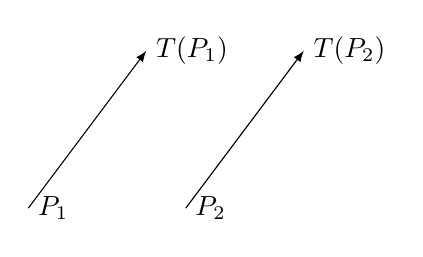
\begin{tikzpicture}[>=latex, scale=1]
        \draw[->] (0,0)node[right]{$P_1$}--(1.5,2)node[right]{$T(P_1)$};
        \draw[->] (2,0)node[right]{$P_2$}--(3.5,2)node[right]{$T(P_2)$};
    \end{tikzpicture}
    \caption{}
    \end{minipage}
    \end{figure}

平面上全体点的一个平移通
常用字母$T$来表示,不同的平移可分别用$T_1,T_2,\ldots$来表示。
如果$P$点通过平移$T$移动到$P_1$点,则$P_1$点叫做$P$点的\textbf{象
点},记作$P_1=T(P)$, 这时有向线段$\Vec{PP_1}$; 可写作$\Vec{PT(P)}$。

为了给出一个平移,根据定义,只需给出平面上任一点
和它的象点即可。设$P_1=T(P)$, 则$P$、$P_1$这两点 就完全
确定了平移$T$的方向和距离;对平面上任一点$A$, 我们都
可作$\Vec{AA_1}=\Vec{PP_1}$, 这样$A$的象点$A_1$也就被$\Vec{PP_1}$所唯一确
定,这也就是说,给定了一个平移$T$, 如果$P_1=T(P)$, 那
么这个平移$T$完全被$\Vec{PT(P)}$所唯一确定,通常我们就用
$\Vec{PT(P)}$或$\Vec{PP_1}$表示这个平移。

显然,平面上全体点的一个移动是一个平移的充要条件
是:对平面上任意两点$P_1$、$P_2$,都有
\[\Vec{P_1T(P_1)}=\Vec{P_2T(P_2)}\]

从以上讨论知,一个平移$T$只有两个要素:\textbf{方向和距离},
因此平面上的一个平移$T$, 可用
那些同向且等长的任一条有向线段来表示。

几次连续平移的结果,叫做平移的\textbf{合成}。设$T_1$、$T_2$是
两次连续平移,这两次连续平移的合成通常记作$T_2\circ T_1$(第
一次平移写在右边),类似地$T_3\circ T_2\circ T_1$, 表示$T_1$、$T_2$、$T_3$三
次连续平移的合成。

\begin{blk}{定理}
    平移的合成还是一个平移且平移的合成满足交换
律。
\end{blk}

\begin{proof}
设$T_1$、$T_2$是两个平移,我们要证明的是:$T_2\circ T_1$也是一个平移,$T_2\circ T_1=T_1\circ T_2$.

设$P$、$Q$是平面上任意两点(图3.5),$P_1=T_1(P)$、
$P_2=T_2(P_1)$、$Q_1=T_1(Q)$、$Q_2=T_2(Q_1)$, 则$P_2=T_2(T_1(P))$, $Q_2=T_2(T_1(Q))$
\begin{figure}[htp]
    \centering
\begin{tikzpicture}[>=latex]
\tkzDefPoints{0/0/P, .85/2/P_1, 2/3/P_2, 4/0/Q}
\tkzDefPointsBy[translation= from P to Q](P_1,P_2){Q_1,Q_2}
\draw[->](P) -- node[left]{$T_1$} (P_1);
\draw[->](Q) -- node[left]{$T_1$} (Q_1);
\draw[->](P) --  (P_2);
\draw[->](Q) -- (Q_2);
\draw[->](P_1) -- node[left]{$T_2$} (P_2);
\draw[->](Q_1) -- node[left]{$T_2$} (Q_2);
\tkzDrawSegments(P,Q P_2,Q_2 P_1,Q_1)
\tkzLabelPoints[left](P_2,Q_2,P_1,Q_1)
\tkzLabelPoints[below](P,Q)
\end{tikzpicture}
    \caption{}
\end{figure}

我们要证明$T_2\circ T_1$是一个平移也就是要证
明$\overline{PP_2}$与$\overline{QQ_2}$平行且等
长。即
\[\Vec{PP_2}=\Vec{QQ_2}\]
由于$T_1$、$T_2$都是平移,则
\[\Vec{PP_1}=\Vec{QQ_1},\qquad \Vec{P_1P_2}=\Vec{Q_1Q_2}\]
连$P$、$P_2$, $Q$、$Q_2$由平行四边形基本定理(即\textbf{一个四边形的
一组对边平行且等长,则另一组对边也平行且等长}),容易
证明:
\[\Vec{PP_2}=\Vec{QQ_2}\]
这就证明了$T_2\circ T_1$也是一个平移。



设点$P$是平面上任一点,$P_1=T_1(P)$, $P_2=T_2(P_1)$,
则$P_2=T_2(T_1(P))$, 这就是说$T_2\circ T_1$把$P$点移动到$P_2$点。

设$Q=T_2(P)$, 由平移定义可知
\[\Vec{P_1P_2}=\Vec{PQ}\]
又由上述平行四边形基本定理可证
\[\Vec{PP_1}=\Vec{QP_2}\]
这就是说
\[P_2=T_1(Q)=T_1(T_2(P))\]
所以
\[T_2\circ T_1=T_1\circ T_2\]
\end{proof}

\begin{figure}[htp]\centering
    \begin{minipage}[t]{0.48\textwidth}
    \centering
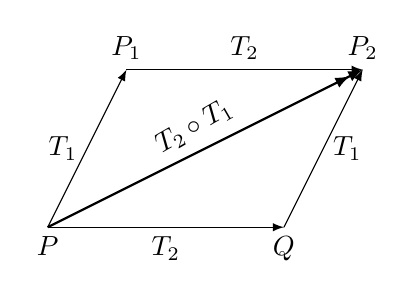
\begin{tikzpicture}[>=latex, scale=1]
    \draw[->](0,0)node[below]{$P$}--node[below]{$T_2$}(3,0) node[below]{$Q$} ;
    \draw[->](0,0)--node[left]{$T_1$}(1,2)node[above]{$P_1$}  ;
    \draw[->](3,0)--node[right]{$T_1$}(4,2)node[above]{$P_2$};
    \draw[->>, thick](0,0)--node[above=1pt, rotate=30]{$T_2\circ T_1$}(4,2)  ;
    \draw[->](1,2)--node[above]{$T_2$}(4,2)  ;
    \end{tikzpicture}
    \caption{}
    \end{minipage}
    \begin{minipage}[t]{0.48\textwidth}
    \centering
    \begin{tikzpicture}[>=latex, scale=.8]
        \draw[->](0,0)--node[below]{$T_1$}(4,0);
        \draw[->](0,0)--node[left]{$T_2$}(0,4);
        \draw[->>](0,0)--node[above, rotate=45]{$5\sqrt{2}$}(4,4);
        \draw[->](4,0)--node[right]{$T_2$}(4,4);
        \draw[->](0,4)--node[above]{$T_1$}(4,4);

        \draw[->](-1,2)--(-1,3)node[left]{北};
    \end{tikzpicture}
    \caption{}
    \end{minipage}
    \end{figure}


\begin{example}
    已知$T_1$表示平移“向东5公里”,$T_2$表示平移
“向北5公里”,求$T_1\circ T_2$, $T_2\circ T_1$.
\end{example}

\begin{solution}
    $T_1\circ T_2=T_2\circ T_1$都表示平移:“向东北$5\sqrt{2}$公里”(图3.7)
\end{solution}

\begin{example}
    已知:$T_1:$ “向东5公里”,$T_2:$ “向西10公里”,求$T_1\circ T_2$和$T_2\circ T_1$.
\end{example}

\begin{solution}
   $T_1\circ T_2=T_2\circ T_1$都表示平移:“向西5公里”(图3.8)。
\end{solution}

\begin{example}
    已知$T_1:$ “向东3公里”,$T_2:$ “向西3公里”,
求$T_1\circ T_2$, $T_2\circ T_1$。
\end{example}

\begin{solution}
    $T_1\circ T_2=T_2\circ T_1$都表示“原地不动”(图3.9)。
这种原地不动的“移动”,可看作平移的特例,叫做\textbf{零平移},零平移记作$\Vec{0}$.
\end{solution}

\begin{blk}
    {定义} 平面上全体点的一个平移,叫做平面上的一个位
移向量,简称向量。
\end{blk}

\begin{figure}[htp]\centering
    \begin{minipage}[t]{0.48\textwidth}
    \centering
\begin{tikzpicture}[>=latex, scale=.9]
\draw[very thick, <->] (2,0)--node[above]{$T_1$}(0,0)--(-2,0);
\draw[thick, ->]  (-4,0)--node[below]{$T_1$}(-2,0);
\draw[thick, ->](-4,0)--(-4,1)node[above]{北};
\draw(0,0)[fill=black]circle (1.5pt);
\draw[thick, ->](2,-.25)--node[below]{$T_2$}(-2,-.25);
\draw[thick, ->](0,.25)--node[above]{$T_2$}(-4,.25);
\draw(-4,0)--(2.5,0);
    \end{tikzpicture}
    \caption{}
    \end{minipage}
    \begin{minipage}[t]{0.48\textwidth}
    \centering
    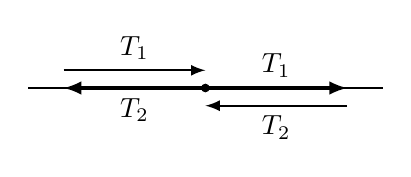
\begin{tikzpicture}[>=latex, scale=.9]
\draw[very thick, <->] (2,0)--node[above]{$T_1$}(0,0)--node[below]{$T_2$}(-2,0);
\draw[thick, ->](2,-.25)--node[below]{$T_2$}(0,-.25);
\draw[thick, ->](-2,.25)--node[above]{$T_1$}(0,.25);
\draw(0,0)[fill=black]circle (1.5pt);
\draw(-2.5,0)--(2.5,0);
    \end{tikzpicture}
    \caption{}
    \end{minipage}
    \end{figure}

如果我们用$\Vec{AB}$, $\Vec{CD}$表示平面上点的平移,我们就说向量$\Vec{AB},\Vec{CD},\ldots$。印刷时
经常用粗体字$\bf{a}$、$\bf{b}$、$\bf{c}$等表
示一个向量。向量$\bf{a}$、$\bf{b}$、$\bf{c}$在
手写时常写作$\vec{a}$、$\vec{b}$、$\vec{c}$。

如果向量$\vec{a}$, 把$A$点移
动到$B$点,$C$点移动到$D$点,$E$点移动到$F$点(图3.10),则
\[\vec{a}=\Vec{AB}=\Vec{CD}=\Vec{EF}=\cdots\]
这些同向且等长的有向线段都表示同一个向量,也就是说它
们中的任一个都可用来表示向量$\vec{a}$。
\begin{figure}[htp]
    \centering
    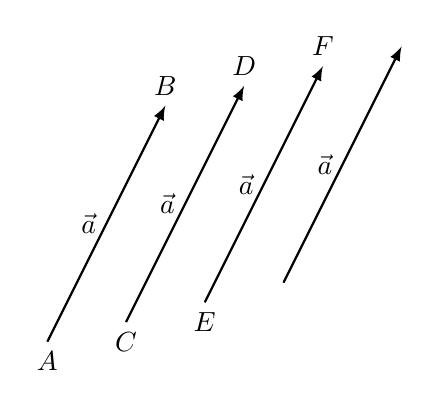
\begin{tikzpicture}[>=latex]
\draw[thick, ->](0,0)node[below]{$A$}--node[left]{$\vec{a}$}(1.5,3)node[above]{$B$};
\draw[thick, ->](1,0.25)node[below]{$C$}--node[left]{$\vec{a}$}(2.5,3.25)node[above]{$D$};
\draw[thick, ->](2,.5)node[below]{$E$}--node[left]{$\vec{a}$}(3.5,3+.5)node[above]{$F$};
\draw[thick, ->](3,.75)--node[left]{$\vec{a}$}(4.5,3+.75);        
    \end{tikzpicture}

    \caption{}
\end{figure}


若$\vec{a}=\Vec{AB}$, 则$\Vec{AB}$的长叫做$\vec{a}$的长度,记作$|\Vec{AB}|$或$|\vec{a}|$.
射线$\Vec{AB}$的方向叫做向量$\vec{a}$的方向。零平移又叫做\textbf{零向量},它
的方向不确定。

如果$\Vec{AB}$与$\Vec{CD}$的方向相同,那么$\Vec{AB}$, $\Vec{CD}$叫做\textbf{同向
向量},如果$\Vec{A_1B_1}$、$\Vec{C_1D_1}$的方向相反,那么$\Vec{A_1B_1}$、$\Vec{C_1D_1}$叫
做\textbf{反向向量}(图3.11)。方向相同或相反的向量,叫做\textbf{平行
向量}。
\begin{figure}[htp]
    \centering
\begin{tikzpicture}[>=latex]
\begin{scope}
    \draw[thick, ->] (0,0)node[below]{$A$}--(0,3)node[above]{$B$};
    \draw[thick, ->] (1,.5)node[below]{$C$}--(1,2.5)node[above]{$D$};    
    \draw[thick, ->] (2,1)--node[left]{$\vec{a}$}(2,3);
\end{scope}
\begin{scope}[xshift=5cm]
    \draw[thick, ->] (0,0)node[below]{$A_1$}--(0,3)node[above]{$B_1$};
    \draw[thick, <-] (1,.5)node[below]{$D_1$}--(1,3)node[above]{$C_1$};    
    \draw[thick, <-] (2,1)--node[left]{$\vec{b}$}(2,2.5);
\end{scope}
\end{tikzpicture}
    \caption{}
\end{figure}

长度为1个单位的向量叫做\textbf{单位向量},通常我们用单位
向量表示平面上的一个方向。

以后我们用到记号$\Vec{AB}$或$\vec{a}$, 它们表示的是一个有向线段
还是一个向量,一般我们都不另加说明,读者可根据实际问
题加以区分。

\begin{ex}
\begin{enumerate}
    \item 用有向线段表示以下平移:
\begin{enumerate}
    \item $T_1$: 向东5cm;
    \item $T_2$: 向南偏西$30^{\circ}$, 3cm;
    \item $T_3$: 向北偏西$60^{\circ}$, 50km.
\end{enumerate}
\item  用有向线段表示以下两个平移的合成:
\begin{enumerate}
    \item $T_1$: 向西5里,$T_2$: 向南3里。
    \item $T_1$: 向北4里,$T_2$: 向西8里。
\end{enumerate}
\end{enumerate}
\end{ex}

\subsection{向量的加法与减法}
向量$\vec{a}$与$\vec{b}$的合成就叫做$\vec{a}$与
$\vec{b}$的和,记作$\vec{a}+\vec{b}$, 即
\[\vec{a}+\vec{b}=\vec{b}\circ \vec{a}\]

由上节定理可知,$\vec{a}$与$\vec{b}$的和$\vec{a}+\vec{b}$也是一个向量。由
于每个向量可由一点和它的象点所唯一确定,所以可按下面
方法作$\vec{a}+\vec{b}$.

在平面上,任取一点$A$ (图3.12), 作$\Vec{AB}=\vec{a}$, $\Vec{BC}=\vec{b}$, 即
$\vec{a}$与$\vec{b}$的合成把$A$点移动到$C$点,因而
\[\Vec{AC}=\vec{a}+\vec{b}\]
\begin{figure}[htp]
    \centering
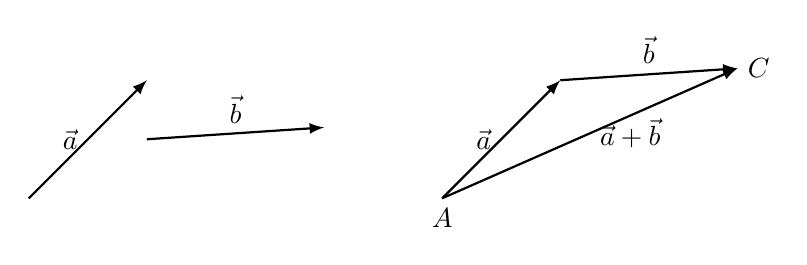
\begin{tikzpicture}[>=latex, scale=1.5]
\begin{scope}
    \draw[->,  thick](0,0)--node[left]{$\vec{a}$}(1,1);
    \draw[->,  thick] (1,.5)--node[above]{$\vec{b}$}(2.5,.6);
\end{scope}

\begin{scope}[xshift=3.5cm]
    \draw[->,  thick](0,0)node[below]{$A$}--node[left]{$\vec{a}$}(1,1);
    \draw[->,  thick](1,1)--node[above]{$\vec{b}$}(2.5,1.1)node[right]{$C$};
    \draw[->,  thick](0,0)--node[right]{$\vec{a}+\vec{b}$}(2.5,1.1);
\end{scope}
\end{tikzpicture}    
    \caption{}
\end{figure}

以上求和作图法叫做\textbf{三角形求和法则}。

由于平移的合成满足交换律,所以向量加法也满足交换
律,即
\[\vec{a}+\vec{b}=\vec{b}+\vec{a}\]

读者不难从图3.13
去验证,向量加法还满
足结合律,即
\[(\vec{a}+\vec{b})+\vec{c}=\vec{a}+(\vec{b}+\vec{c})\]
\begin{figure}[htp]\centering
    \begin{minipage}[t]{0.48\textwidth}
    \centering
\begin{tikzpicture}[>=latex,scale=1.5]
    \tkzDefPoints{0/0/A, 1/1.5/B, 3/1.7/C, 3.5/0/D}
\draw[->, thick](A)--node[left]{$\vec{a}$}(B);
\draw[->, thick](A)--node[above,rotate=30]{$\vec{a}+\vec{b}$}(C);
\draw[->, thick](A)--node[below]{$(\vec{a}+\vec{b})+\vec{c}=\vec{a}+(\vec{b}+\vec{c})$}(D);
\draw[->, thick](B)--node[above]{$\vec{b}$}(C);
\draw[->, thick](B)--node[above,rotate=-35]{$\vec{b}+\vec{c}$}(D);
\draw[->, thick](C)--node[right]{$\vec{c}$}(D);
    \end{tikzpicture}
    \caption{}
    \end{minipage}
    \begin{minipage}[t]{0.48\textwidth}
    \centering
    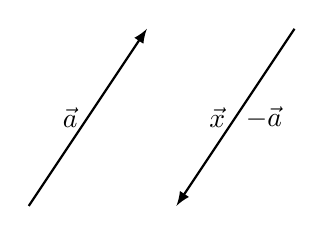
\begin{tikzpicture}[>=latex, scale=1.5]
      \draw[->, thick](0,0)--node[left]{$\vec{a}$}(1,1.5);
      \draw[<-, thick](1.25,0)--node[left]{$\vec{x}$}node[right]{$-\vec{a}$}(2.25,1.5);
    \end{tikzpicture}
    \caption{}
    \end{minipage}
    \end{figure}

容易看出,$\vec{a}+\vec{0}=\vec{0}+\vec{a}=\vec{a}$.

如果向量$\vec{a}$与$\vec{x}$反向且等长,那么由求和作图法可知
(图3.14)
\[\vec{a}+\vec{x}=\vec{0}\]

如果用$-\vec{a}$表示$\vec{x}$, 那么$-\vec{a}$叫
做$\vec{a}$的\textbf{逆向量}或\textbf{负向量},于是
\[\vec{a}+(-\vec{a})=\vec{0}\]
如图3.15所示。



\begin{example}
    

\end{example}

\begin{solution}
    
\end{solution}

\begin{example}
    



\end{example}

\begin{solution}
    
\end{solution}

\begin{solution}
    
\end{solution}

























































